\documentclass[spanish]{beamer}
\mode<presentation>
\usepackage[utf8]{inputenc}
\usepackage[spanish]{babel}

\usepackage{default}
\usecolortheme{orchid}
\usetheme{Goettingen}
\usefonttheme{professionalfonts}

\usepackage{multicol}
\usepackage{textcomp}


\usepackage{color}
\usepackage{listings}
\usepackage{graphicx}
\usepackage{float}

\definecolor{mygreen}{rgb}{0,0.6,0}
\definecolor{mygray}{rgb}{0.5,0.5,0.5}
\definecolor{mymauve}{rgb}{0.58,0,0.82}
%\hypersetup{pdfpagemode=FullScreen}

\title[Contribuyendo a Python]{Contribuyendo a Python}
\author{Arias Emmanuel}
\institute[Flisol 2019]{15º Festival Latinoamericano de Instalación de Software Libre}
\date{La Rioja,  27 de abril 2019}

\begin{document}
\lstset{
	language=Python,
    showspaces=false,
	numbers=left,
	keywordstyle=\color{blue},
	numbersep=5pt,
	numberstyle=\color{mygray},
	rulecolor=\color{black},
	stringstyle=\color{mymauve}}

\begin{frame}
	\titlepage
	
\includegraphics[width=0.5\textwidth]{flisol.png}
	
\includegraphics[width=0.5\textwidth]{pyar.png}
\end{frame}

\section{¿Por qué Contribuir al Software Libre?}
\begin{frame}
 \begin{center}
	 ¿Por qué contribuir al Software Libre (y open source)? 
 \end{center}
\end{frame}

\section{Python}
\begin{frame}
	\frametitle{Python}
	\begin{itemize}
		\item Creado por Guido van Rossum.
		\item Lenguaje de programación interpretado y de propósito general.
		\item Tipado dinámico, multiplataforma.
		\item Código abierto.
		\item Nace con la filosofía de ser fácil de aprender, que su implementación
			sea veloz y que el código escrito sea legible.
	\end{itemize}
\end{frame}

\begin{frame}[fragile]
	\frametitle{Ejemplo en Python}
	\begin{lstlisting}
	print("Hello World")
	\end{lstlisting}
\end{frame}

\begin{frame}[fragile]
	\frametitle{Ejemplo en C}
	\begin{lstlisting}[language=c]
	#include <stdio.h>

	int main(int argc, char* argv[]){
	    printf("Hello World");
	    return 0;
	}
	\end{lstlisting}

\end{frame}

\begin{frame}[fragile]
	\frametitle{Ejemplo en Java}
	\begin{lstlisting}[language=java]
public class HelloWorld {
    public static void main(String[] args) {
    System.out.println("Hello, World");
    }
}
        \end{lstlisting}
\end{frame}

\begin{frame}
	\frametitle{Entonces Python...}
	\begin{itemize}
		\item Es un lenguaje multi paradigma:
			\begin{itemize}
				\item Programación Orientada a Objeto
				\item Programación estructurada
				\item Programación funcional
			\end{itemize}
		\item Puede ser ejecutado a través de un archivo .py y además,
			a través de un modo interactivo del intérprete.
	\end{itemize}
\end{frame}

\section{¿Python es un lenguaje nuevo?}
\begin{frame}
	\frametitle{¿Python es un lenguaje nuevo?}
	\begin{itemize}
		\item Guido van Rossum comenzo el desarrollo de Python en
			diciembre de 1989, como un hobbie.
		\item En 1991 tuvo su primera release (0.9.0). En 1994 se lanza
			la versión 1.0. En 2000 surge la versión 2.0 y en 2008
			se libera la versión 3.0.
		\item JavaScript, Java (JDK Beta) y Ruby tienen su primera release en 1995.
	\end{itemize}
\end{frame}

\section{Pero, y ¿cómo puedo contribuir?}
\begin{frame}
	\frametitle{Pero, y cómo puedo contribuir?}
	¿Necesito ser un gran desarrollador? 
        \begin{figure}
		\centering
		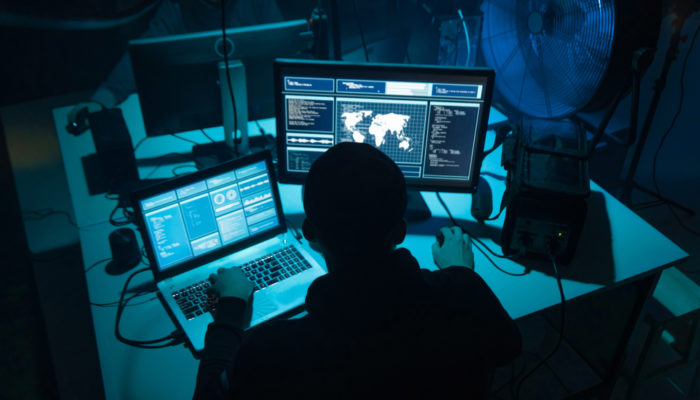
\includegraphics[width=1\linewidth]{image1.jpg}
	\end{figure}
\end{frame}

\subsection{PSF}
\begin{frame}
	\frametitle{Python Software Foundation}
	\begin{itemize}
		\item La PSF tiene como misión promover, proteger y hacer avanzar el 
			lenguage de programación Python.
		\item Da soporte al crecimiento de una comunidad diversa e internacional
			de programadores Python.
		\item Existen varios proyectos bajo la infraestructura de la fundación:
			\begin{itemize}
				\item CPython
				\item pythondotorg
				\item devguide
				\item bedevere
				\item miss-islington
				\item blurb\_it
			\end{itemize}
		\item https://www.python.org/psf-landing/
	\end{itemize}
\end{frame}

\subsubsection{CPython}
\begin{frame}
	\frametitle{CPython}
	\begin{itemize}
		\item Es el interprete ``oficial'' escrito en C. 
		\item Existen otros interpretes implementados en diferentes lenguajes:
			\begin{itemize}
				\item Jython (Java)
				\item IronPython (.Net)
				\item MicroPython (Python para microcontroladores)
				\item PyPy (interprete de Python escrito en Python)
			\end{itemize}
	\end{itemize}
\end{frame}
\begin{frame}
	\frametitle{CPython (devguide)}
	\begin{itemize}
		\item Un buen lugar para comenzar es leyendo la Python Developer's Guide
			(https://devguide.python.org/)
	\end{itemize}
	\center
	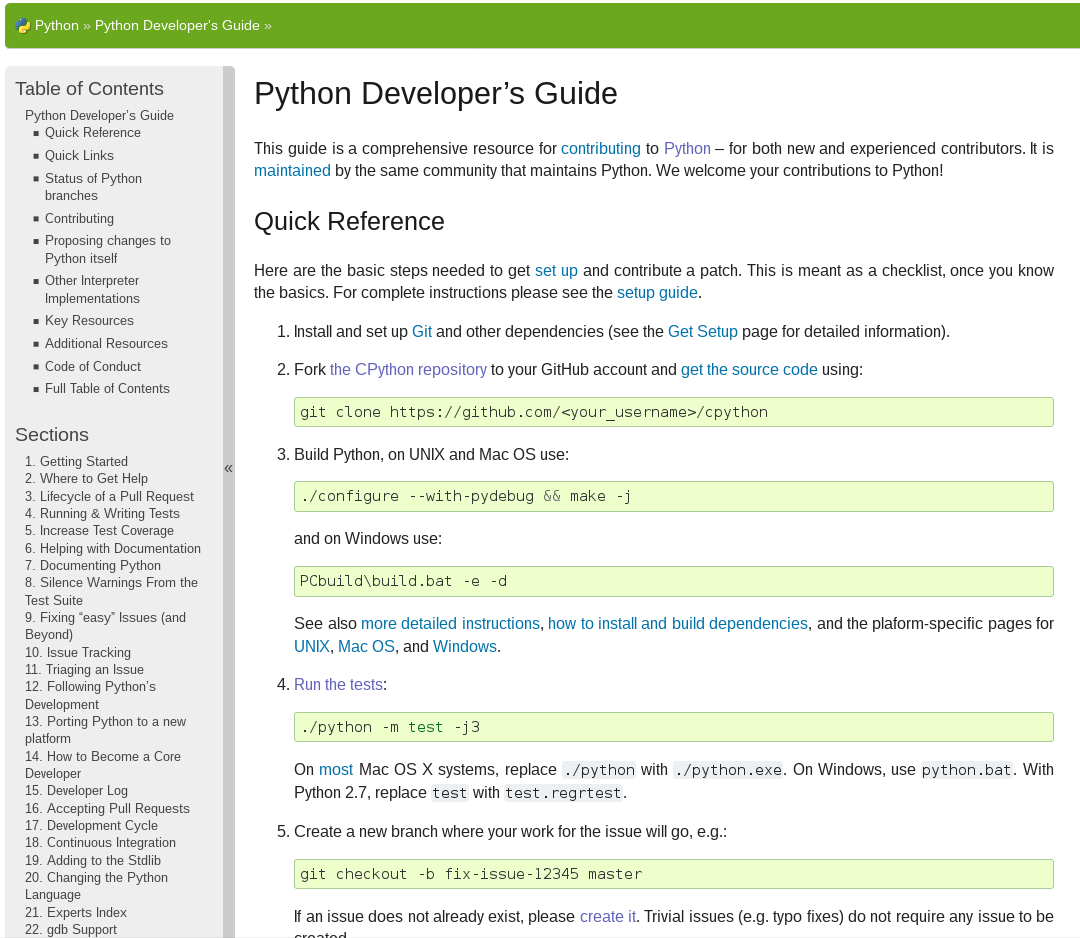
\includegraphics[width=1\linewidth]{devguide.png}
\end{frame}
\begin{frame}
	\frametitle{CPython - Consiguiendo el código}
	\begin{itemize}
		\item Con una cuenta de Github se debe hacer un fork del repositorio de CPython.
	\end{itemize}
	\center
	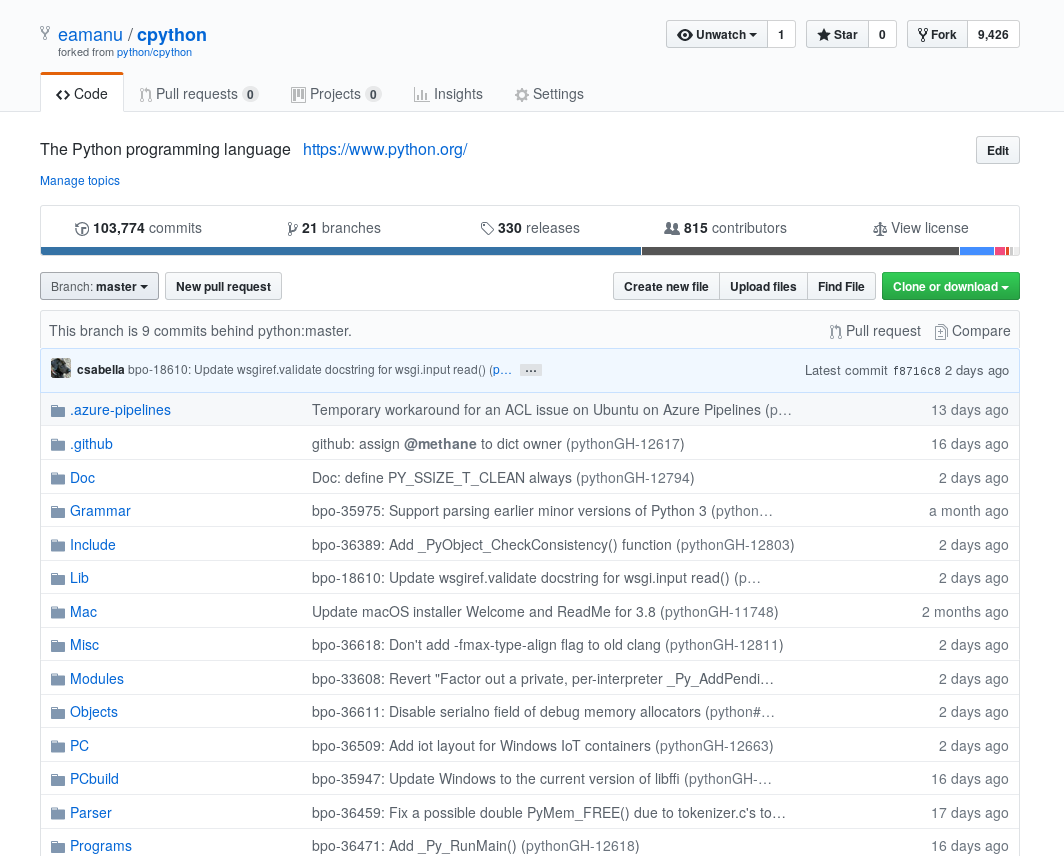
\includegraphics[width=0.8\linewidth]{fork.png}
\end{frame}

\begin{frame}[fragile]
	\frametitle{CPython - Consiguiendo el código}
	\begin{lstlisting}[language=bash]
git clone git@github.com:eamanu/cpython.git
	\end{lstlisting}

	\center
	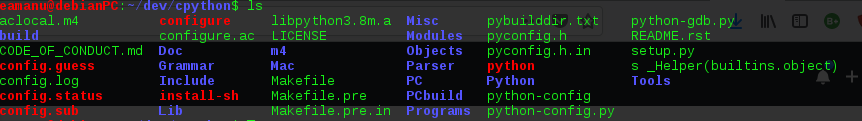
\includegraphics[width=0.8\linewidth]{clone.png}
\end{frame}

\begin{frame}
	\frametitle{CPython -  Resolviendo bugs}

\end{frame}

\end{document}
